\documentclass[10pt,landscape]{article}
\usepackage{multicol}
\usepackage{calc}
\usepackage{ifthen}
\usepackage[landscape]{geometry}
\usepackage{listings}
\usepackage{amsmath,amsthm,amsfonts,amssymb}
\usepackage{mathtools}
\usepackage{color,graphicx,overpic}
\usepackage{hyperref}
\usepackage[table, dvipsnames, xcdraw]{xcolor} % for \colorbox and named colors
\usepackage{transparent}

\usepackage{MnSymbol}
\usepackage{graphicx}
\usepackage{wrapfig}
\usepackage{tikz}

\usepackage{blindtext}

% This sets page margins to .1 inch if using letter paper, and to 1cm
% if using A4 paper. (This probably isn't strictly necessary.)
% If using another size paper, use default 1cm margins.
\ifthenelse{\lengthtest { \paperwidth = 11in}}
    { \geometry{top=0.2in,left=0.2in,right=0.2in,bottom=0.2in} }
    {\ifthenelse{ \lengthtest{ \paperwidth = 297mm}}
        {\geometry{top=1cm,left=1cm,right=1cm,bottom=1cm} }
        {\geometry{top=1cm,left=1cm,right=1cm,bottom=1cm} }
    }

% Turn off header and footer
\pagestyle{empty}

% Redefine section commands to use less space
\makeatletter
\renewcommand{\section}{\@startsection{section}{1}{0mm}%
                                {-1ex plus -.5ex minus -.2ex}%
                                {0.5ex plus .2ex}%x
                                {\normalfont\large\bfseries}}
\renewcommand{\subsection}{\@startsection{subsection}{2}{0mm}%
                                {-1ex plus -.5ex minus -.2ex}%
                                {0.5ex plus .2ex}%
                                {\normalfont\normalsize\bfseries}}
\renewcommand{\subsubsection}{\@startsection{subsubsection}{3}{0mm}%
                                {-1ex plus -.5ex minus -.2ex}%
                                {0.5ex plus .2ex}%
                                {\normalfont\footnotesize\bfseries}}
\makeatother

% Itemize to use less space
\usepackage{enumitem}
\setlist{leftmargin=*, nosep}
\setenumerate{nosep}

% Define BibTeX command
\def\BibTeX{{\rm B\kern-.05em{\sc i\kern-.025em b}\kern-.08em
    T\kern-.1667em\lower.7ex\hbox{E}\kern-.125emX}}

% Don't print section numbers
\setcounter{secnumdepth}{0}


\setlength{\parindent}{0pt}
\setlength{\parskip}{0pt plus 0.5ex}

%My Environments
\newtheorem{example}[section]{Example}

\newcommand{\Blue}[1]{\noindent{\textcolor{Blue}{\textbf{#1}}}:}
\newcommand{\Red}[1]{\noindent{\textcolor{BrickRed}{\textbf{#1}}}:}
\newcommand{\Green}[1]{\noindent{\textcolor{PineGreen}{\textbf{#1}}}:}
\newcommand{\Hint}[1]{\noindent{\textcolor{Orange}{#1}}}

\newcommand{\TODO}[1]{%
  \vspace{1em}%
  \noindent\textbf{\Large\textcolor{BrickRed}{TODO: #1}}%
  \vspace{1em}%
}

\newcommand*{\eg}{e.g.\@\xspace}
\newcommand*{\ie}{i.e.\@\xspace}
\newcommand*{\Eg}{E.g.\@\xspace}
\newcommand*{\Ie}{I.e.\@\xspace}
\newcommand*{\esp}{esp.\@\xspace}
\newcommand*{\wrt}{\ifmmode \stext{w.r.t.} \else w.r.t.\@\xspace \fi}


\usepackage{draftwatermark}
% Configure the watermark
\SetWatermarkText{Made with love by \texttt{junruren}} % Set the watermark text
\SetWatermarkScale{0.35}            % Adjust the scale of the watermark
\SetWatermarkLightness{0.9}      % Set the lightness (closer to 1 is more faded)
% -----------------------------------------------------------------------

\begin{document}
\raggedright
\scriptsize

\begin{multicols}{4}
% multicol parameters
% These lengths are set only within the two main columns
%\setlength{\columnseprule}{0.25pt}
\setlength{\premulticols}{1pt}
\setlength{\postmulticols}{1pt}
\setlength{\multicolsep}{1pt}
\setlength{\columnsep}{2pt}

\subsection{Diversification}

\subsubsection{Asset return characteristics}

Buy an asset (\eg a stock) at $t = 0$ at price $P_0$. At time $t = 1$,
\begin{itemize}
    \item its cash flow (dividend) is $D_1$, and
    \item its price is $P_1$
\end{itemize}
(both are random variables). The risk-free rate is $r_F$.

\Blue{Realized return}
\fbox{$r_1 = \frac{D_1 + P_1}{P_0} - 1$}
Returns comes from both dividends and capital gains.

\Blue{Expected return}
\fbox{$E[r_1] = \frac{E[D_1] + E[P_1]}{P_0} - 1$}

\Blue{Excess return} (realized)
\fbox{$r_1 - r_F$}

\Blue{Risk premium} (expected excess return) \fbox{$E[r_1] - r_F$}

\Red{Mean (average) return}
\fbox{$\bar{r} = E[r] = \frac{1}{T} \sum_{t=1}^T r_t$}
Would be same as the expected return $E[r_t]$ if expected returns are constant for all $t$.

\Blue{Estimate Expected Return}
\begin{itemize}
    \item if have multiple possible scenarios for returns and know the probability of each scenario, use:
    \fbox{$E[r] = \sum_{i=1}^N p_i r_i$}
    \item if have a time series of past $T$ observations of returns, estimate sample estimate of expected return $\bar{r}$ as:
    \fbox{$\hat{r} = \frac{1}{T} \sum_{t=1}^T r_t$}
\end{itemize}

\Red{Variance} measures the volatility or deviation of returns from the mean.
\fbox{$\text{Var}(r) = \sigma^2 = E\left[(r - E[r])^2\right]$}
If given (past) data sample of $T$ returns, the sample variance is:
\fbox{$\hat{\sigma}^2 = \frac{1}{T-1} \sum_{t=1}^T (r_t - \bar{r})^2$}
where the expected return $\bar{r}$ can be estimated by the sample mean $\bar{r}$ as defined above.

\Red{Standard deviation} \fbox{$\sigma = \sqrt{\text{Var}(r)}$} measures the risk of the asset. Gives a magnitude in percent.

\Red{Covariance} measures the degree to which two random variables move together.
\fbox{$\sigma_{ij} = \text{Cov}(r_i, r_j) = E[(r_i - \bar{r_i})(r_j - \bar{r_j})]$}

\Blue{Estimate Cov} given (past) data sample of $T$ returns, the sample covariance is:
\fbox{$\hat{\sigma}_{ij} = \frac{1}{T-1} \sum_{t=1}^T (r_{i,t} - \bar{r_i})(r_{j,t} - \bar{r_j})$}

Covariance can be:
\begin{itemize}
    \item positive (\Hint{both variables move in the same direction}),
    \item negative (\Hint{two variables move in the opposite direction}), or
    \item zero (no relationship).
\end{itemize}
\Hint{Variance is a special case of covariance, where the two variables are the same.}
\fbox{$\text{Var}(r_i) = \sigma_{ii} = \text{Cov}(r_i, r_i)$}

\Red{Correlation} measures the strength of the linear relationship between two random variables.
\Hint{Always between -1 and 1.}
\fbox{$\text{Corr}(r_i, r_j) = \rho_{ij} = \frac{\text{Cov}(r_i, r_j)}{\sigma_i \sigma_j}$}

\Red{Beta} measures the sensitivity of an asset's return to the return of the market portfolio.
\fbox{$\beta_i = \frac{\text{Cov}(r_i, r_m)}{\text{Var}(r_m)}$}
where $r_m$ is the return of the market portfolio.

Other measures of risk:
\begin{itemize}
    \item \Blue{Skewness} captures the asymmetry of the distribution of returns.
    \item \Blue{Kurtosis} captures the "tailedness" of the distribution of returns. Higher kurtosis means more extreme values (outliers) in the distribution. \ie the distribution has ``fat tails''.
\end{itemize}

\Red{Mean-variance investors} care about the expected return (higher is better) and variance (lower is better) of the return. They are risk-averse with a risk-aversion coefficient of $A$.
\Blue{Mean-variance utility function} captures the preferences of mean-variance investors
\fbox{${U(r) = E[r] - \frac{1}{2} A \cdot \text{Var}(r)}$} where $U(r)$ is the utility of the return $r$.

\Blue{Indifference curve} is a curve that represents all combinations of expected return and variance that give the same utility to the investor. The slope of the indifference curve is given by:
\fbox{$\frac{dE[r]}{d\sigma^2} = -A$}
The slope is negative, meaning that as variance increases, the expected return must also increase to maintain the same utility.

\subsubsection{Portfolio}

\Red{Portfolio} a combination of different assets or securities. Defined by number $N_i$ and the price $P_i$ of each asset $i$ in the portfolio. The total value of the portfolio is:
\fbox{$V = \sum_{i=1}^n N_i P_i$}

\Blue{Portfolio weight} of asset $i$ in the portfolio is:
\fbox{$w_i = \frac{N_i P_i}{V}$}
The portfolio weight represents the proportion of the total portfolio value that is invested in asset $i$.
Weights can be \Hint{positive (long position)} or \Hint{negative (short position)}. $\sum_{i=1}^{n} w_i = 1$

\Red{Mean and variance of a portfolio} with weights: $w_1, \dots, w_n$ and returns $r_1, \dots, r_n$:
\begin{itemize}
    \item \Blue{Random variable} $R_p = \sum_{i=1}^n w_i r_i$
    \item \Blue{Expected return}
    \fbox{$E[R_p] = \sum_{i=1}^N w_i E[r_i]$}
    \item \Blue{Variance}
    \fbox{$\text{Var}(R_p) = \sum_{i=1}^n \sum_{j=1}^n w_i w_j \text{Cov}(r_i, r_j)$}
\end{itemize}
\Green{Special case - two assets}
\begin{itemize}
    \item $E[R_p] = w_1 E[r_1] + w_2 E[r_2]$
    \item $\text{Var}(R_p) = w_1^2 \text{Var}(r_1) + w_2^2 \text{Var}(r_2) + 2 w_1 w_2 \text{Cov}(r_1, r_2)$ (\Hint{Note: $w_2 = 1 - w_1$})
\end{itemize}

\Green{Special case - $n$ equally-weighted assets} with returns $r_1, \dots, r_n$:
\begin{itemize}
    \item $E[R_p] = \frac{1}{n} \sum_{i=1}^n E[r_i]$
    \item $\text{Var}(R_p) = \frac{1}{n^2} \sum_{i=1}^n \sum_{j=1}^n \text{Cov}(r_i, r_j)$
\end{itemize}

\Blue{Portfolio beta} is the sensitivity of the portfolio return to the return of the market portfolio.

\Red{Efficient frontier and the tangency portfolio}
\begin{itemize}
    \item \Blue{Mean-variance frontier portfolio} minimizes risk (measured by variance) for a given expected return.
    \item \Blue{Efficient frontier} is the set of portfolios that offer the highest expected return for a given level of risk. (Upper part of the mean-variance frontier)
    \item \Blue{Sharpe ratio}
    \fbox{$= \frac{E[R_p] - r_f}{\sigma_p}$}
    is the slope of the line from the risk-free rate to the portfolio. It measures the risk-adjusted return of the portfolio.
    \item \Blue{Capital Market Line} represents the risk-return trade-off of efficient portfolios. It starts at the risk-free rate and is tangent to the efficient frontier. The slope of the CML is equal to the Sharpe ratio of the tangency portfolio.
\end{itemize}

\subsection{Options}

\Red{Options}
Derivative contracts specifying \textbf{a right} to \textbf{buy (call option)} or \textbf{sell (put option)} an underlying asset at a specified price $K$ (the \textbf{strike/exercise price}) on or before a specified date $T$ (the \textbf{expiration/maturity date}).

\begin{itemize}
    \item \Blue{Call option}: right to buy the underlying asset at the strike price.
    \item \Blue{Put option}: right to sell the underlying asset at the strike price.
\end{itemize}

Exercise style:
\begin{itemize}
    \item \Blue{American option}: can be exercised at any time before expiration.
    \item \Blue{European option}: can only be exercised at expiration.
\end{itemize}

\subsubsection{Option Payoff curves}

\begin{itemize}
    \item \Blue{$S$} Price of the underlying asset at expiration
    \item \Blue{$K$} Strike price of option
    \item \Hint{Payoff $\neq$ Profit}. To get profit (net payoff), need to subtract the option's cost.
\end{itemize}

\begin{multicols}{2}
\tiny \textbf{Payoff of buying a Call}
$\max(0, S - K)$
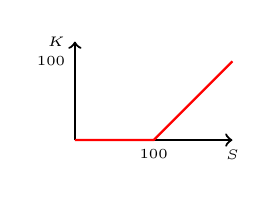
\begin{tikzpicture}
    % Draw lines
    \draw[->,thick] (0,0) -- (2,0) node[anchor=north] {\tiny $S$}; % Asset Price axis
    \draw[->,thick] (0,0) -- (0,1.25) node[anchor=east] {\tiny $K$}; % Strike Price axis
    % Draw payoff lines
    \draw[-,thick,red] (0,0) -- (1,0) -- (2,1);

    % Label values
    \node[anchor=north] at (1,0) {\tiny $100$};
    \node[anchor=east] at (0,1) {\tiny $100$};
\end{tikzpicture}

\tiny \textbf{Payoff of buying a Put}
$\max(0, K - S)$
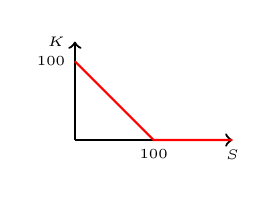
\begin{tikzpicture}
    % Draw lines
    \draw[->,thick] (0,0) -- (2,0) node[anchor=north] {\tiny $S$}; % Asset Price axis
    \draw[->,thick] (0,0) -- (0,1.25) node[anchor=east] {\tiny $K$}; % Strike Price axis
    % Draw payoff lines
    \draw[-,thick,red] (0,1) -- (1,0) -- (2,0);

    % Label values
    \node[anchor=north] at (1,0) {\tiny $100$};
    \node[anchor=east] at (0,1) {\tiny $100$};
\end{tikzpicture}

\tiny \textbf{Payoff of selling a Call}
$-\max(0, S - K)$
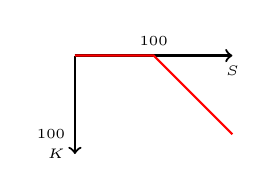
\begin{tikzpicture}
    % Draw lines
    \draw[->,thick] (0,0) -- (2,0) node[anchor=north] {\tiny $S$}; % Asset Price axis
    \draw[->,thick] (0,0) -- (0,-1.25) node[anchor=east] {\tiny $K$}; % Strike Price axis
    % Draw payoff lines
    \draw[-,thick,red] (0,0) -- (1,0) -- (2,-1);

    % Label values
    \node[anchor=south] at (1,0) {\tiny $100$};
    \node[anchor=east] at (0,-1) {\tiny $100$};
\end{tikzpicture}

\tiny \textbf{Payoff of selling a Put}
$-\max(0, K - S)$
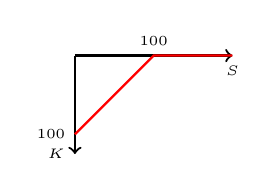
\begin{tikzpicture}
    % Draw lines
    \draw[->,thick] (0,0) -- (2,0) node[anchor=north] {\tiny $S$}; % Asset Price axis
    \draw[->,thick] (0,0) -- (0,-1.25) node[anchor=east] {\tiny $K$}; % Strike Price axis
    % Draw payoff lines
    \draw[-,thick,red] (0,-1) -- (1,0) -- (2,0);

    % Label values
    \node[anchor=south] at (1,0) {\tiny $100$};
    \node[anchor=east] at (0,-1) {\tiny $100$};
\end{tikzpicture}
\end{multicols}

Payoff curves of other assets that can be used with options:
\begin{multicols}{2}
\tiny Payoff of underlying asset
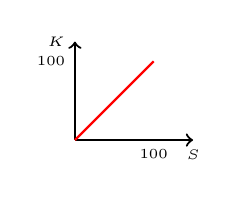
\begin{tikzpicture}
    % Draw lines
    \draw[->,thick] (0,0) -- (1.5,0) node[anchor=north] {\tiny $S$}; % Asset Price axis
    \draw[->,thick] (0,0) -- (0,1.25) node[anchor=east] {\tiny $K$}; % Strike Price axis
    % Draw payoff lines
    \draw[-,thick,red] (0,0) -- (1,1);

    % Label values
    \node[anchor=north] at (1,0) {\tiny $100$};
    \node[anchor=east] at (0,1) {\tiny $100$};
\end{tikzpicture}

\tiny Payoff of a \$100 FV ZC Bond
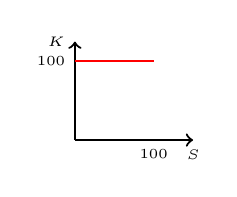
\begin{tikzpicture}
    % Draw lines
    \draw[->,thick] (0,0) -- (1.5,0) node[anchor=north] {\tiny $S$}; % Asset Price axis
    \draw[->,thick] (0,0) -- (0,1.25) node[anchor=east] {\tiny $K$}; % Strike Price axis
    % Draw payoff lines
    \draw[-,thick,red] (0,1) -- (1,1);

    % Label values
    \node[anchor=north] at (1,0) {\tiny $100$};
    \node[anchor=east] at (0,1) {\tiny $100$};
\end{tikzpicture}
\end{multicols}

\subsubsection{Option payoff and profit}

\begin{itemize}
    \item \Blue{$r$} Risk-free interest rate (EAR)
    \item \Blue{$C$} Call option price
    \item \Blue{$P$} Put option price
\end{itemize}

\Blue{Call option}
\begin{tabular}{c|c|c|c}
    & $S < K$ & $S = K$ & $S > K$ \\
    \hline
    Payoff & $0$ & $0$ & $S - K$ \\
    Profit & $-C (1+r)^T$ & $-C (1+r)^T$ & $S - K - C (1+r)^T$ \\
\end{tabular}

\Blue{Put option}
\begin{tabular}{c|c|c|c}
    & $S < K$ & $S = K$ & $S > K$ \\
    \hline
    Payoff & $K - S$ & $0$ & $0$ \\
    Profit & $K - S - P(1+r)^T$ & $- P(1+r)^T$ & $- P(1+r)^T$ \\
\end{tabular}

An option is
\begin{itemize}
    \item \Blue{in-the-money} if it has positive payoff at expiration. A call option is in-the-money if $S > K$, and a put option is in-the-money if $S < K$.
    \item \Blue{out-of-the-money} if it has zero payoff at expiration. A call option is out-of-the-money if $S < K$, and a put option is out-of-the-money if $S > K$.
    \item \Blue{at-the-money} if it has zero payoff at expiration. A call option is at-the-money if $S = K$, and a put option is at-the-money if $S = K$.
\end{itemize}

\Red{Put-call parity} following portfolios have the same payoff at expiration:
\begin{enumerate}
    \item \Blue{Long call with strike price $K$ + Bond with face value $K$}

    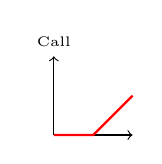
\begin{tikzpicture}
        % Draw lines
        \draw[->] (0,0) -- (1,0); % Asset Price axis
        \draw[->] (0,0) -- (0,1) node[anchor=south] {\tiny Call}; % Strike Price axis
        % Draw payoff lines
        \draw[-,thick,red] (0,0) -- (0.5,0) -- (1,0.5);
    \end{tikzpicture}
    \raisebox{4ex}{+}
    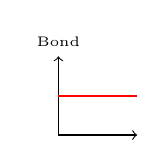
\begin{tikzpicture}
        % Draw lines
        \draw[->] (0,0) -- (1,0); % Asset Price axis
        \draw[->] (0,0) -- (0,1) node[anchor=south] {\tiny Bond}; % Strike Price axis
        % Draw payoff lines
        \draw[-,thick,red] (0,0.5) -- (1,0.5);
    \end{tikzpicture}
    \raisebox{4ex}{=}
    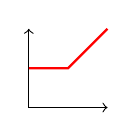
\begin{tikzpicture}
        % Draw lines
        \draw[->] (0,0) -- (1,0); % Asset Price axis
        \draw[->] (0,0) -- (0,1); % Strike Price axis
        % Draw payoff lines
        \draw[-,thick,red] (0,0.5) -- (0.5,0.5) -- (1,1);
    \end{tikzpicture}
    \item \Blue{Long put with strike price $K$ + Underlying asset}

    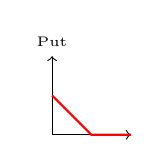
\begin{tikzpicture}
        % Draw lines
        \draw[->] (0,0) -- (1,0); % Asset Price axis
        \draw[->] (0,0) -- (0,1) node[anchor=south] {\tiny Put}; % Strike Price axis
        % Draw payoff lines
        \draw[-,thick,red] (0,0.5) -- (0.5,0) -- (1,0);
    \end{tikzpicture}
    \raisebox{4ex}{+}
    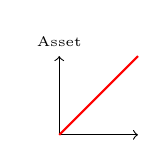
\begin{tikzpicture}
        % Draw lines
        \draw[->] (0,0) -- (1,0); % Asset Price axis
        \draw[->] (0,0) -- (0,1) node[anchor=south] {\tiny Asset}; % Strike Price axis
        % Draw payoff lines
        \draw[-,thick,red] (0,0) -- (1,1);
    \end{tikzpicture}
    \raisebox{4ex}{=}
    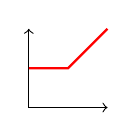
\begin{tikzpicture}
        % Draw lines
        \draw[->] (0,0) -- (1,0); % Asset Price axis
        \draw[->] (0,0) -- (0,1); % Strike Price axis
        % Draw payoff lines
        \draw[-,thick,red] (0,0.5) -- (0.5,0.5) -- (1,1);
    \end{tikzpicture}
\end{enumerate}

Given their identical payoffs, under no-arbitrage, they should have the same price:
\begin{itemize}
    \item $P_{call} + P_{bond} = P_{put} + P_{asset}$
    \item $C + K(1+r)^{-T} = P + S$
\end{itemize}

\Red{Binomial option pricing model} Iterative approach to price options that makes the following simplifications:
\begin{itemize}
    \item Discrete periods, in which stock price can either go up or down.
    \item We find the option price by a \textit{no arbitrage} argument. Price is equal to the cost of purchasing a \textit{replicating portfolio} whose payoffs match the option payoff in each state. \Eg, for a call, we solve: $\begin{cases}
        a S_u + b B_u &= C_u \\
        a S_d + b B_d &= C_d
    \end{cases}$ where $a$ is the number of shares of stock, $b$ is the number of bonds, $S_u$ and $S_d$ are the stock prices if it goes up or down, and $C_u$ and $C_d$ are the call option prices if stock goes up or down.
    \item  Under the binomial assumptions, \Hint{the probability of a stock moves up or down is irrelevant}, and the price of options can be determined solely using: \begin{itemize}
        \item Current stock price $S_0$, interest rate $r$, strike price $K$ and time to maturity $T$;
        \item Magnitude of possible future changes of stock price (volatility), captured implicitly by the possible values the stock can take $S_u$ and $S_d$.
    \end{itemize}
\end{itemize}

\Red{Black-Scholes formula} Taking the limit of binomial model as the number of periods gets large, we obtain the B-S formula for the price of a European call option without dividends:
\fbox{$C(S, K, T, r, \sigma) = S \cdot N(x) - K(1 + r)^{-T} \cdot N(x - \sigma \sqrt{T})$}
\begin{itemize}
    \item \Blue{$S$} current value of the underlying asset (in \$)
    \item \Blue{$K$} strike price of the option (in \$)
    \item \Blue{$T$} option maturity (in years)
    \item \Blue{$r$} annual risk-free interest rate
    \item \Blue{$\sigma$} annualized standard deviation of the underlying asset's return (volatility)
    \item \Blue{$N(\cdot)$} cumulative normal distribution function (\texttt{NORM.S.DIST(x, TRUE)}). These $N(\cdot)$ terms \Hint{capture the replicating portfolio weights}.
    \item \Blue{$x$} \fbox{$x = \frac{\ln\left(\frac{S}{K(1+r)^{-T}}\right)}{\sigma \sqrt{T}} + \frac{1}{2} \sigma \sqrt{T}$}
\end{itemize}

\subsubsection{Real options}
Option-like payoffs appear in many contexts outside of financial markets. Management can be thought of as the act of creating and optimally exercising real options. \Green{\Eg} follow-on products, R\&D  investments, delaying product launches, abandoning projects, etc.

\end{multicols}
\end{document}